\subsection{LM IFU: integral-field spectroscopy}
\label{ssec:overview_ifu}

% The \ac{IFU} pipeline has not yet been revised since PDR, hence the
% description in \cite{DRLS} applies.
% For reference, t
The association map is shown in Fig.~\ref{Fig:IfuAssomap}.

% Discussion moved to https://github.com/AstarVienna/METIS_DRLD/issues/100
% \TODO{
% We will consider rearranging the recipes to be in line with the
% imaging pipelines. This would entail handling basic reduction and
% background subtraction for of both science and standard exposures in
% common recipes (\CODE{metis_ifu_basic}, \CODE{metis_ifu_background}),
% then having a recipe to analyse the standard observations
% (\CODE{metis_ifu_std_process}). The science exposures are then fully
% calibrated (\CODE{metis_ifu_calibrate}). A full set of exposures would
% then be assembled and restored with a fully sampled PSF in a
% post-processing recipe (\CODE{metis_ifu_combine}).
% }

\begin{landscape}
\begin{figure}[ht]
  \centering
  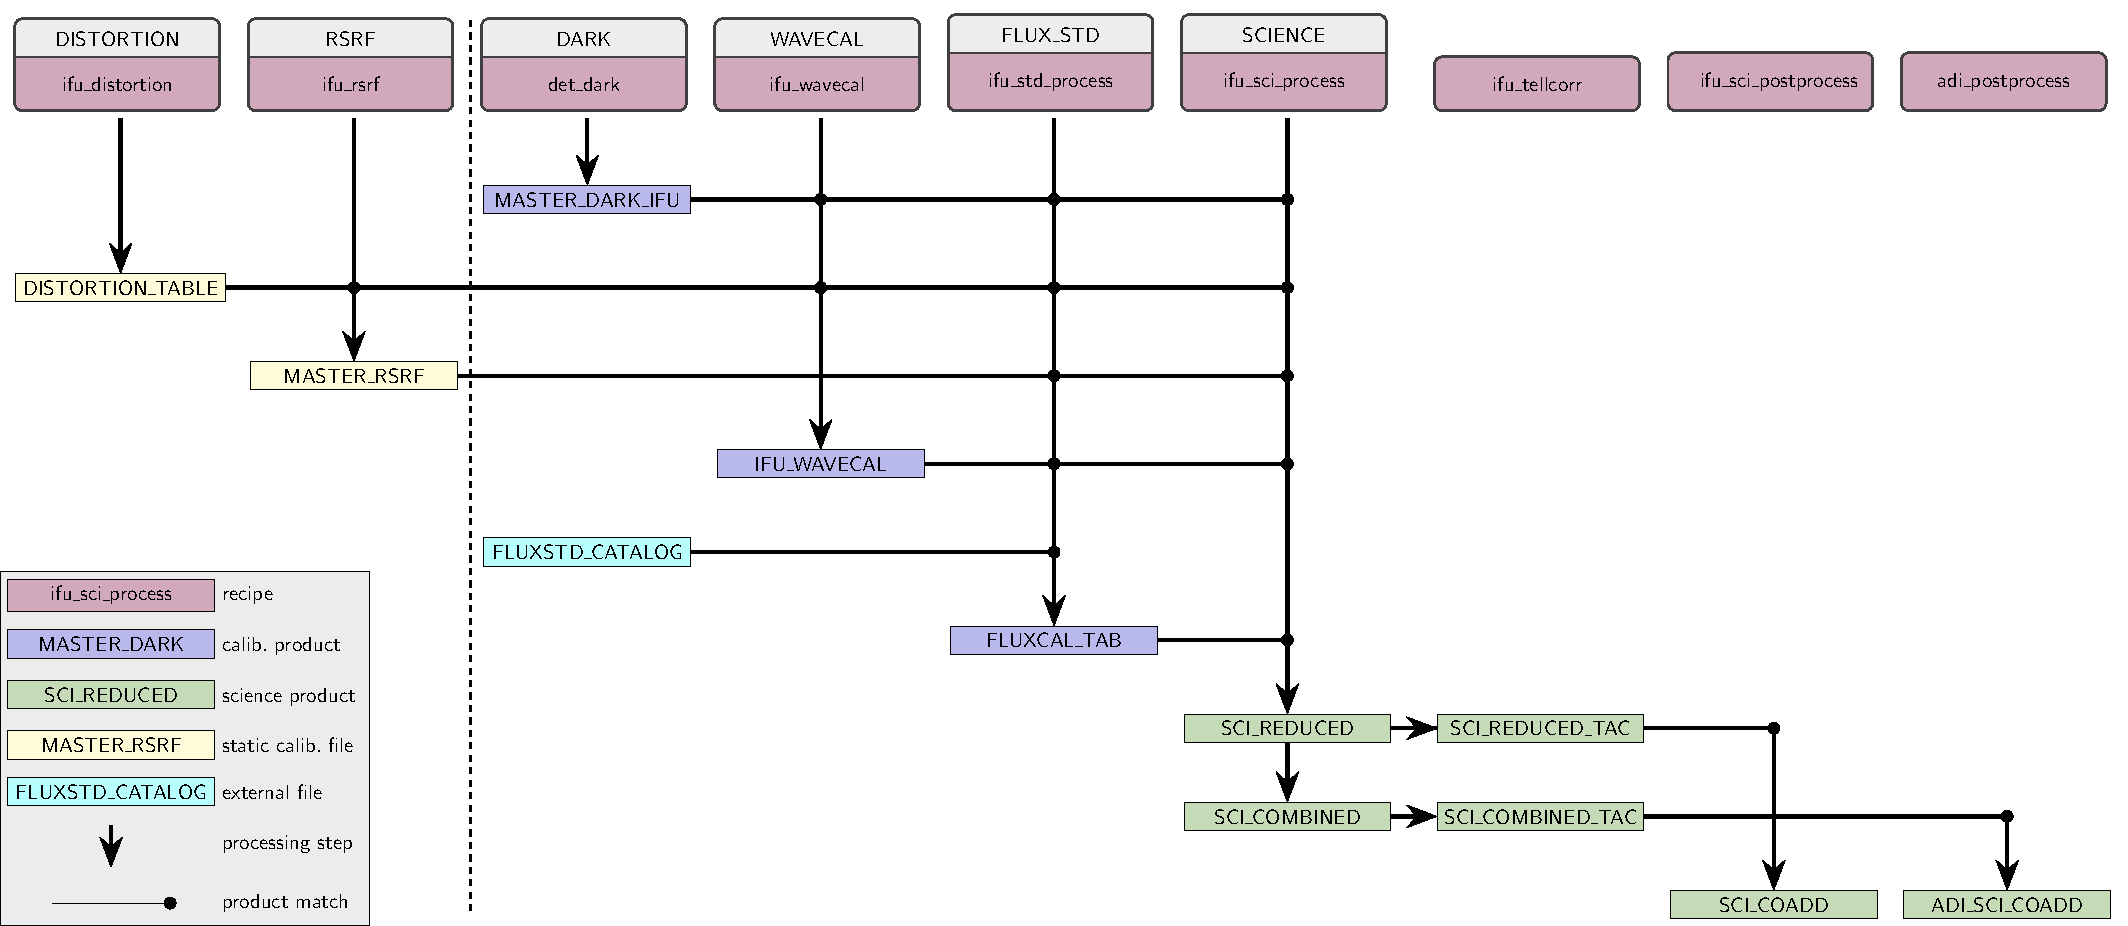
\includegraphics{IFU_assomap_tikz}
  \caption[Reduction cascade and association map for IFU
  spectroscopy]{%
    Association map for \ac{IFU} spectroscopy in L- and M-band. The
    figure shows only the primary products created by each recipe; for
    a full list of products refer to the recipe descriptions in
    Sect.~\ref{ssec:IFU_recipes}. The dashed line separates
    calibration tasks that are done at AIT or infrequently during
    operations from tasks done daily. The prefix ``\REC{metis_}'' has been
    omitted from the recipe names to improve clarity.}
  \label{Fig:IfuAssomap}
\end{figure}
\end{landscape}



%%%%%%%%%%%%%%%%%%%%%%%%%%%%%%%%%%%%%%%%%%%%%%%%%%%%%%

%%% Local Variables:
%%% TeX-master: "METIS_DRLD"
%%% End:
